% Matches MS Word: A4, 12pt Times New Roman, Narrow margins (1.27 cm all round).
\documentclass[12pt,a4paper]{article}
\usepackage[margin=1.27cm]{geometry}
\linespread{1.0}
\usepackage{mathptmx}          % Times New Roman for text and maths
\usepackage{graphicx,booktabs,amsmath,amssymb,xcolor,float,multirow,capt-of}
\usepackage[font=footnotesize,labelfont=bf,skip=1.5pt]{caption}
\usepackage[compact]{titlesec}
\usepackage{enumitem}
\usepackage[hidelinks]{hyperref}
\usepackage{tikz}
\usetikzlibrary{arrows.meta,positioning,calc}

\titlespacing*{\section}{0pt}{3pt}{0.5pt}
\titlespacing*{\subsection}{0pt}{3pt}{0.5pt}
\titleformat{\section}{\normalfont\large\bfseries}{}{0em}{}
\titleformat{\subsection}{\normalfont\normalsize\bfseries}{}{0em}{}
\setlist[itemize]{leftmargin=1.1em,itemsep=0pt,topsep=0.5pt,parsep=0pt}
\setlist[enumerate]{leftmargin=1.4em,itemsep=0pt,topsep=0.5pt,parsep=0pt}
\setlength{\parskip}{0.8pt}
\setlength{\abovedisplayskip}{2.5pt}
\setlength{\belowdisplayskip}{2.5pt}
\setlength{\abovedisplayshortskip}{1pt}
\setlength{\belowdisplayshortskip}{1pt}
\setlength{\textfloatsep}{2.5pt}
\setlength{\intextsep}{2pt}
\renewcommand{\arraystretch}{0.88}
\captionsetup[table]{skip=1pt}
\newcommand{\D}{\mathcal{D}}
\renewcommand{\topfraction}{0.92}
\renewcommand{\bottomfraction}{0.7}
\renewcommand{\textfraction}{0.06}
\renewcommand{\floatpagefraction}{0.85}
\newcommand{\file}[1]{\textcolor{gray}{\small\texttt{#1}}}

\begin{document}
\pagestyle{plain}

\begin{center}
{\large\bfseries COMP6010 Assignment: From Bayesian Inference to Generative AI}\\[1pt]
{\small Planning and Handling Uncertainty in Machine Learning}\\[2pt]
{\bfseries Satria Pamungkas} \quad\textbullet\quad ID: {\bfseries 21522611}
\quad\textbullet\quad Part C option: {\bfseries C2} (animal drawings, flow matching)
\end{center}
\vspace{-3pt}\hrule\vspace{2pt}

\noindent\textbf{Introduction.} This report answers three questions using probability. Part~A does
\emph{inference}: the model is fully known, and the job is to use evidence correctly. Part~B \emph{learns}
one unknown number, and shows why a decision must use the whole posterior instead of a single best guess.
Part~C \emph{learns a generative model} --- a flow-matching network trained from scratch on Quick, Draw!
drawings --- showing the same pattern works when the unknown is a whole function. Every number comes from
the supplement's notebooks and is saved in a named file, shown in \file{grey type}. The unit materials [1]
are the primary source throughout.

\section{Part A: Bayesian network simulation and sampling}

\subsection{A1. The model and exact answers}

Five yes/no variables: $H$ (hot weather), $F$ (irrigation fault), $D$ (dry soil), $S$ (sensor says
``dry''), $W$ (plants wilting). Arrows are $H\!\to\!D$, $F\!\to\!D$, $D\!\to\!S$, $D\!\to\!W$,
$H\!\to\!W$. The two causes at the top are independent, with $P(H{=}1)=0.30$ and $P(F{=}1)=0.08$.

\begin{minipage}[t]{0.26\textwidth}
\vspace{1pt}\centering
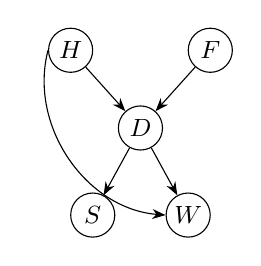
\begin{tikzpicture}[>=Stealth,node distance=7mm and 7mm,
  every node/.style={circle,draw,minimum size=5.6mm,inner sep=0pt,font=\small}]
\node (H) {$H$};
\node (F) [right=12mm of H] {$F$};
\node (D) [below=7mm of $(H)!0.5!(F)$] {$D$};
\node (S) [below left=7mm and 2mm of D] {$S$};
\node (W) [below right=7mm and 2mm of D] {$W$};
\draw[->] (H) -- (D); \draw[->] (F) -- (D);
\draw[->] (D) -- (S); \draw[->] (D) -- (W);
\draw[->] (H.west) to[bend right=50] (W.west);
\end{tikzpicture}
\end{minipage}%
\begin{minipage}[t]{0.73\textwidth}
\vspace{3pt}
The arrows split the joint probability into one small piece per variable:
\[P(H,F,D,S,W)=P(H)\,P(F)\,P(D\mid H,F)\,P(S\mid D)\,P(W\mid H,D).\]
That is $2{+}2{+}4{+}2{+}4$ table entries instead of the 31 numbers a full joint over five yes/no variables
would need --- the graph is what saves that work.

One independence the graph gives is $S \perp W \mid D,H$: the sensor connects to the network only through
$D$, its single parent, so once we know $D$ (and $H$, which also feeds $W$) the sensor tells us nothing new
about wilting. Checked in code: $\max|P(S\mid D,H,W)-P(S\mid D,H)|<10^{-16}$.
\end{minipage}

\smallskip
Listing all $2^5=32$ states gives a total probability of 1 (to within $2\times10^{-16}$) and the exact
answers in Table~\ref{tab:Aexact}. Two more checks matter. First, adding up the right states returns
$P(H{=}1)=0.30$ and $P(F{=}1)=0.08$, and $P(H{=}1,F{=}1)=P(H{=}1)P(F{=}1)$, so the two causes really
are independent before any evidence. Second, and more useful: I purposely swapped the $H$ and $F$
columns in the $D$ table to plant a bug. The total \emph{still} added to 1, so checking the total alone
would have missed it --- but $q_1$ changed from $0.2315$ to $0.2044$, so checking the answers caught
it. Getting the total right is necessary but nowhere near enough.
\file{A1\_exact\_reference\_values.csv}

\begin{table}[H]\centering\small
\caption{Exact answers found by listing all 32 states. The last column shows why rare evidence makes
rejection sampling slow.}
\label{tab:Aexact}
\begin{tabular}{llrrr}
\toprule
Query & Meaning & Exact answer & $P(\text{evidence})$ & Samples kept per 1{,}000 \\
\midrule
$q_1$ & $P(F{=}1\mid S{=}1)$ & 0.231504 & 0.26816 & 268 \\
$q_2$ & $P(F{=}1\mid S{=}1,W{=}1)$ & 0.293294 & 0.15932 & 159 \\
$q_3$ & $P(F{=}1\mid S{=}1,W{=}1,H{=}1)$ & 0.168675 & 0.10956 & 110 \\
\bottomrule
\end{tabular}
\end{table}

\subsection{A2. Forward sampling and rejection sampling}

To draw a yes/no variable $X$ with $P(X{=}1\mid\text{parents})=p$, pick a random number $u$ evenly
between 0 and 1 and set $x=1$ if $u<p$. This works because $u$ is spread evenly, so the chance of landing
below $p$ is exactly $p$: picture the line from 0 to 1 cut at $p$, where the two piece lengths \emph{are}
the two probabilities. I must pick the right table row first using the parent values already drawn, which
is why the loop follows $(H,F,D,S,W)$ --- parents always come first, so the finished samples are genuine
draws from the exact joint.

Rejection sampling throws away every sample that disagrees with the evidence and reports the share
of survivors with $F{=}1$. This is correct because ``restrict to the cases where the evidence
happened'' and ``condition on the evidence'' mean the same thing; the price is that only a fraction
$P(e)$ survive. I generate one sample set per seed and reuse it for all three queries, at
$N\in\{10^3,10^4,10^5\}$ with five seeds each. Survival rates match Table~\ref{tab:Aexact} well (e.g.\
$0.1590$ against $0.15932$ for $q_2$ at $N{=}10^5$). No answer was undefined across the 45 runs --- the
fewest survivors was 107, for $q_3$ at $N{=}10^3$ --- but the code returns \texttt{NaN} for a $0/0$
case rather than inventing a number.
\file{A2\_rejection\_per\_run.csv}

\subsection{A3. Likelihood weighting}

I implemented likelihood weighting only, since the brief warns against adding Gibbs sampling just to write
more code. The evidence variables are \emph{forced} to their observed values, the rest are drawn as usual in
parent-first order, and each sample gets a weight
$w=\prod_{E_i\in\mathcal{E}}P(E_i{=}e_i\mid\mathrm{pa}(E_i))$, giving the weighted average
$\hat P(F{=}1\mid e)=\sum_{k:F^{(k)}=1}w^{(k)}\big/\sum_k w^{(k)}$.

\textbf{Why the weights are needed.} Forcing the evidence means drawing from the wrong distribution
$Q$, not the posterior. Since $P(x_{-\mathcal{E}}\mid e)=Q(x_{-\mathcal{E}})\,w(x_{-\mathcal{E}})/P(e)$,
the weight is exactly the correction between the two: it gives
$\mathbb{E}_Q[w\,\mathbb{1}(F{=}1)]=P(F{=}1,e)$ and $\mathbb{E}_Q[w]=P(e)$, so dividing one by the other
gives the answer. Counting \emph{without} weights just returns the prior --- I measured $0.0800$ against
the true $q_2=0.2933$ --- because forcing a variable \emph{below} $F$ cannot change how $F$ was drawn.
The weights are the only thing carrying evidence back up the arrows. Dividing must use $\sum_k w^{(k)}$,
which estimates $P(e)$ (average weight $0.1600$ against the true $0.159316$); dividing by $N$ would give
$P(F{=}1,e)$ instead. Note $H$ in $q_3$ sits at the top of the graph, so it only contributes the fixed
$0.30$ --- only evidence with parents makes the weights vary. \file{A3\_likelihood\_weighting\_per\_run.csv}

\subsection{A4. Comparing the two methods}

\begin{figure}[H]\centering
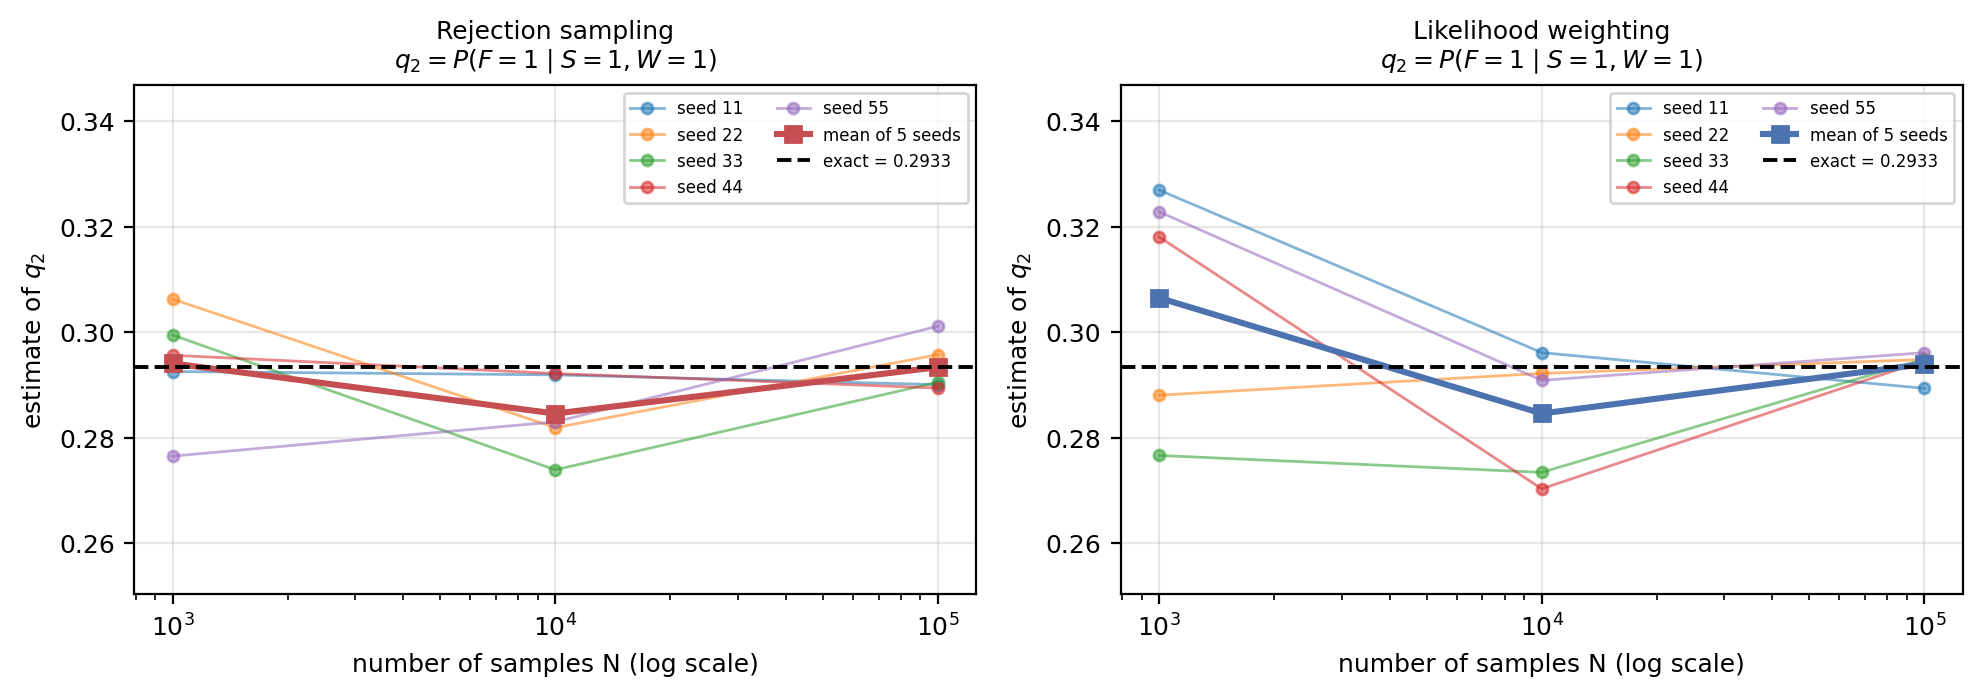
\includegraphics[width=0.50\textwidth]{../Satria_Pamungkas_21522611_COMP6010_Supplement/results/partA/A4_convergence_q2.png}
\hfill
\begin{minipage}[b]{0.40\textwidth}
\small
\captionof{table}{Average $\pm$ spread over five seeds.}
\label{tab:Acmp}
\vspace{-2pt}
\begin{tabular}{@{}llll@{}}
\toprule
 & $N$ & Rejection & Lik.\ weighting \\
\midrule
$q_1$ & $10^3$ & .238$\pm$.014 & .251$\pm$.040 \\
      & $10^4$ & .228$\pm$.007 & .227$\pm$.009 \\
      & $10^5$ & .231$\pm$.003 & .231$\pm$.002 \\
$q_2$ & $10^3$ & .294$\pm$.011 & .307$\pm$.023 \\
      & $10^4$ & .285$\pm$.008 & .285$\pm$.012 \\
      & $10^5$ & .293$\pm$.005 & .294$\pm$.003 \\
$q_3$ & $10^3$ & .170$\pm$.019 & .173$\pm$.016 \\
      & $10^4$ & .161$\pm$.018 & .167$\pm$.004 \\
      & $10^5$ & .169$\pm$.005 & .169$\pm$.001 \\
\bottomrule
\end{tabular}
\end{minipage}
\caption{How $q_2$ settles down as $N$ grows (five seeds; the dashed line is the exact answer). Both
methods head to the right value, and the spread shrinks in step with $1/\sqrt{N}$.
\file{A4\_convergence\_q2.png}, \file{A4\_summary\_table.csv}}
\label{fig:Aconv}
\end{figure}

\textbf{What each new piece of evidence does.} Start from the prior $P(F{=}1)=0.08$. A ``dry'' reading
lifts this to $q_1=0.2315$, about 2.9 times the prior, but still low: the sensor is only 90\% accurate,
and dry soil has a likelier rival cause, since hot weather starts at $0.30$ against the fault's $0.08$.
Adding wilting raises it to $q_2=0.2933$, because wilting is a \emph{second and separate} sign of dry
soil --- $S\perp W\mid D,H$ means the two are separate measurements of the same hidden thing, so it
backs the sensor up instead of repeating it. Adding hot weather pushes the answer back \emph{down} to
$q_3=0.1687$. This is \textbf{explaining away}: $D$ has two parents, so confirming one good rival cause
makes the other less necessary. In plain terms, a dry-soil alert on a hot day is much weaker evidence
of a fault than the same alert on a cool day. These are probabilities under the model we were given,
not proof about a real greenhouse. \file{A4\_evidence\_sequence.csv}

\textbf{Accuracy against effort.} Rejection sampling keeps only a fraction $P(e)$ of its samples, so
every extra piece of evidence shrinks what is left: at $N{=}10^5$ it keeps about 26{,}800 samples for
$q_1$ but only 10{,}900 for $q_3$, while likelihood weighting keeps all $N$. With the five seeds the
brief asks for, this is \emph{not} reliably visible --- rejection sampling wins a few rows in
Table~\ref{tab:Acmp} --- so I ran an extra check with 400 seeds. Likelihood weighting then has the
smaller spread and error in \textbf{9 out of 9} (query, $N$) combinations, by about $1.04$--$1.26$ times
for $q_1$ and $q_2$ and a steady $2.05$ times for $q_3$. Five seeds are simply not enough to rank two
methods this close. On whether a few weights dominate, the effective sample size [9]
$\mathrm{ESS}=(\sum w)^2/\sum w^2$ divided by $N$ gives $0.40$, $0.22$ and $0.46$: the weight takes only
a few values here and the largest 1\% hold under 6\% of the total, so no small group takes over --- true
for this small network with mild evidence, not in general. One fair-comparison note: rejection sampling
makes one sample set shared by all three queries, while likelihood weighting reruns per evidence set, so
I time them separately rather than pretending a ``sample'' means the same work in both.
\file{A4\_variance\_check\_400seeds.csv}, \file{A4\_timing.csv}

\textbf{Why more samples do not always help.} Each estimate is itself random. A bigger $N$ shrinks how
much it \emph{varies}, so the error falls on average and the seeds bunch closer --- but a single run can
get lucky at small $N$. For $q_2$ with rejection sampling, seeds 11 and 33 got \emph{worse} from
$N{=}10^3$ to $10^4$, and seeds 11 and 44 from $10^4$ to $10^5$. Only averaged results say anything
about a method; one run does not. That is exactly why five seeds are required.

\textbf{Why forcing later evidence is wrong.} Forward sampling draws each variable from
$P(x_i\mid\mathrm{pa}_i)$, so influence only flows parent to child; overwriting an observed child afterwards
cannot change how its parents were drawn. I tried it: forcing $S{=}1,W{=}1$ across 200{,}000 samples gave
$0.0799$ --- the prior --- instead of $q_2=0.2933$. Diagnosis runs \emph{against} the arrows, so a fix is
compulsory: throw away samples that disagree (rejection), or reweight by how likely the evidence was.

\section{Part B: learning with a Beta prior}

\subsection{B1. Setting up the problem}

Each grasp either works or it does not, so the Bernoulli distribution fits: it is the only distribution on
$\{0,1\}$ and has one parameter, $P(X_i{=}x\mid\theta)=\theta^x(1-\theta)^{1-x}$. For $n$ independent attempts
with $s$ successes the likelihood is $\theta^s(1-\theta)^{n-s}$, depending on the data only through $s$ and $n$.

The parameter $\theta$ is not something we observe. It is an unknown \emph{continuous} number between
0 and 1, so describing our uncertainty needs a curve (a density), not one value. The Beta family lives
exactly on the interval 0 to 1 --- the right range for a probability. The key convenience is
\textbf{conjugacy}: the Beta formula $\theta^{\alpha-1}(1-\theta)^{\beta-1}$ has the same shape as the
Bernoulli likelihood, so multiplying them gives another Beta, and updating becomes arithmetic on two
numbers. Note $\alpha$ and $\beta$ are \emph{prior settings, not data}: they act like $\alpha{-}1$
pretend successes and $\beta{-}1$ pretend failures, so $\mathrm{Beta}(2,3)$ is a slightly pessimistic
starting belief (average $0.4$) worth about three real attempts.

\begin{minipage}[t]{0.27\textwidth}
\vspace{0pt}\centering
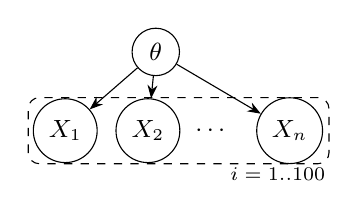
\begin{tikzpicture}[>=Stealth,font=\small]
\node[circle,draw,minimum size=6mm] (th) at (0,0) {$\theta$};
\node[circle,draw,minimum size=5.6mm] (x1) at (-1.15,-1.0) {$X_1$};
\node[circle,draw,minimum size=5.6mm] (x2) at (-0.1,-1.0) {$X_2$};
\node at (0.72,-1.0) {$\cdots$};
\node[circle,draw,minimum size=5.6mm] (xn) at (1.7,-1.0) {$X_{n}$};
\draw[->] (th) -- (x1); \draw[->] (th) -- (x2); \draw[->] (th) -- (xn);
\draw[dashed,rounded corners] (-1.62,-1.42) rectangle (2.2,-0.58);
\node[font=\scriptsize] at (1.55,-1.55) {$i=1..100$};
\end{tikzpicture}
\end{minipage}%
\begin{minipage}[t]{0.69\textwidth}
\vspace{3pt}
$\theta$ is the one shared parent of every observation, so
$f(\theta,x_1..x_n)=f(\theta)\prod_i P(x_i\mid\theta)$ and $X_i \perp X_j \mid \theta$: once $\theta$ is
fixed, knowing attempt 3 succeeded says nothing about attempt 4. But the attempts are \emph{not}
independent before we know $\theta$. By simulation, under the prior $P(X_2{=}1\mid X_1{=}1)=0.4283$ while
$P(X_2{=}1\mid X_1{=}0)=0.3335$; hold $\theta$ fixed and both become $0.55$. This shared-parent link is
what \emph{makes learning possible} --- if attempts were independent from the start, data could never
teach us about $\theta$. Note too that a density is not a probability: $f(0.8)$ can exceed 1 while
$P(\theta{=}0.8)=0$ exactly, which is why B3 asks for an area, not a height.
\end{minipage}

\subsection{B2. Updating the posterior}

Putting the Bernoulli likelihood and Beta prior into Bayes' rule, and sweeping every factor that does
not contain $\theta$ into the constant:
\[
f(\theta\mid\D)\;\propto\;\underbrace{\theta^{s}(1-\theta)^{n-s}}_{\text{likelihood}}\cdot
\underbrace{\theta^{\alpha-1}(1-\theta)^{\beta-1}}_{\text{prior}}
=\theta^{(\alpha+s)-1}(1-\theta)^{(\beta+n-s)-1}
\;\Longrightarrow\;
\theta\mid\D\sim\mathrm{Beta}(\alpha+s,\;\beta+n-s).
\]
So updating means: add successes to $\alpha$, failures to $\beta$. Updating batch by batch and updating once
with the totals \emph{must} agree, because the likelihood multiplies across batches and multiplication ignores
order. Both give $\mathrm{Beta}(2{+}85,\,3{+}15)=\mathbf{Beta(87,18)}$, checked by assertion. I also compared
the shortcut against Bayes' rule computed numerically on a 200{,}001-point grid (largest difference about
$10^{-9}$) and confirmed all six batch orders agree.
\file{B2\_sequential\_updates.csv}

\begin{table}[H]\centering\small
\caption{Running estimates. All three move together as the data (100 attempts) swamps the prior
(worth about 3 attempts). \file{B2\_point\_estimates.csv}}
\label{tab:Bpoint}
\begin{tabular}{lrrrrrr}
\toprule
Stage & Posterior & Total $n$ & Total $s$ & ML $s/n$ & Posterior mean & MAP \\
\midrule
Prior & $\mathrm{Beta}(2,3)$ & 0 & 0 & --- & 0.4000 & 0.3333 \\
After batch 1 & $\mathrm{Beta}(8,7)$ & 10 & 6 & 0.6000 & 0.5333 & 0.5385 \\
After batch 2 & $\mathrm{Beta}(24,11)$ & 30 & 22 & 0.7333 & 0.6857 & 0.6970 \\
After batch 3 & $\mathrm{Beta}(87,18)$ & 100 & 85 & 0.8500 & \textbf{0.8286} & 0.8350 \\
\bottomrule
\end{tabular}
\end{table}

The distance between the posterior mean and the ML estimate shrinks from $0.067$ after batch 1 to $0.021$ after
batch 3 --- the prior pulls hardest when data are scarce. MAP sits between the two because this posterior leans
left, so its peak is above its average.

\subsection{B3. Uncertainty and the deployment decision}

Three different quantities, all from $\mathrm{Beta}(87,18)$:

\textbf{(1) Prediction for the next attempt.} We do not know $\theta$, so instead of plugging in a guess we
average over every value it might take:
$P(X_{n+1}{=}1\mid\D)=\int_0^1\theta\,f(\theta\mid\D)\,d\theta=\mathbb{E}[\theta\mid\D]=\mathbf{0.8286}$. The
\emph{number} matches the posterior mean, but the ideas differ --- one is about a future observation, the other
summarises a curve --- and they agree only because averaging is a straight-line operation. For anything curved
they part ways: the chance the next \emph{two} attempts both succeed is $\mathbb{E}[\theta^2]=0.6879$, above
$(\mathbb{E}[\theta])^2=0.6865$, so plugging in the average understates it.

\textbf{(2) 95\% credible interval:} $[\mathbf{0.7512},\,\mathbf{0.8941}]$, checked by confirming the cumulative
probability is $0.025$ at the bottom and $0.975$ at the top.

\textbf{(3) Probability above the threshold:} $P(\theta>0.8\mid\D)=\mathbf{0.7883}$, checked two ways
--- numerical integration agrees with SciPy [3] to eight decimal places, and 200{,}000 random draws from
the posterior (seed \texttt{20260910}) give $0.78688$, within half a standard error.

\textbf{The decision: the rule is NOT met.} It needs $P(\theta>0.8\mid\D)\ge0.95$ and we have $0.7883$, short
by $0.1617$; at the same success rate, roughly 400--500 more attempts would be needed to pass.

\textbf{Why a good point estimate is not enough.} Both the ML estimate $(0.8500)$ and the posterior
mean $(0.8286)$ are \emph{above} $0.8$, and the rule still fails. A single number throws away how wide
the posterior is: after 100 attempts the curve still has real width (spread $0.0366$) and $21.2\%$ of
it sits below $0.8$. The interval agrees --- its lower end, $0.7512$, is under the threshold, so
$\theta<0.8$ is not ruled out. The rule is written about the whole curve on purpose, because the cost of
a bad gripper is paid when $\theta$ really is low, not when the average looks fine. To pass, the
posterior must be \emph{packed} above $0.8$, not merely centred above it.

\textbf{Why the height of the curve at 0.8 is not this probability.} $f(0.8)=7.26$ is a density --- a rate of
probability per unit of $\theta$ --- so it cannot be compared with $0.95$; this curve even peaks at $10.96$,
far above 1, and any single exact value has probability zero for a continuous quantity. What the rule needs is
the \emph{area} right of $0.8$. The notebook shows the link: the probability of landing within $\pm0.0005$ of
$0.8$ is $0.0072565$, and the height times that width is $0.0072556$ --- precisely what a density means.
\file{B3\_decision.json}, \file{B3\_mc\_verification.png}

\begin{figure}[H]\centering
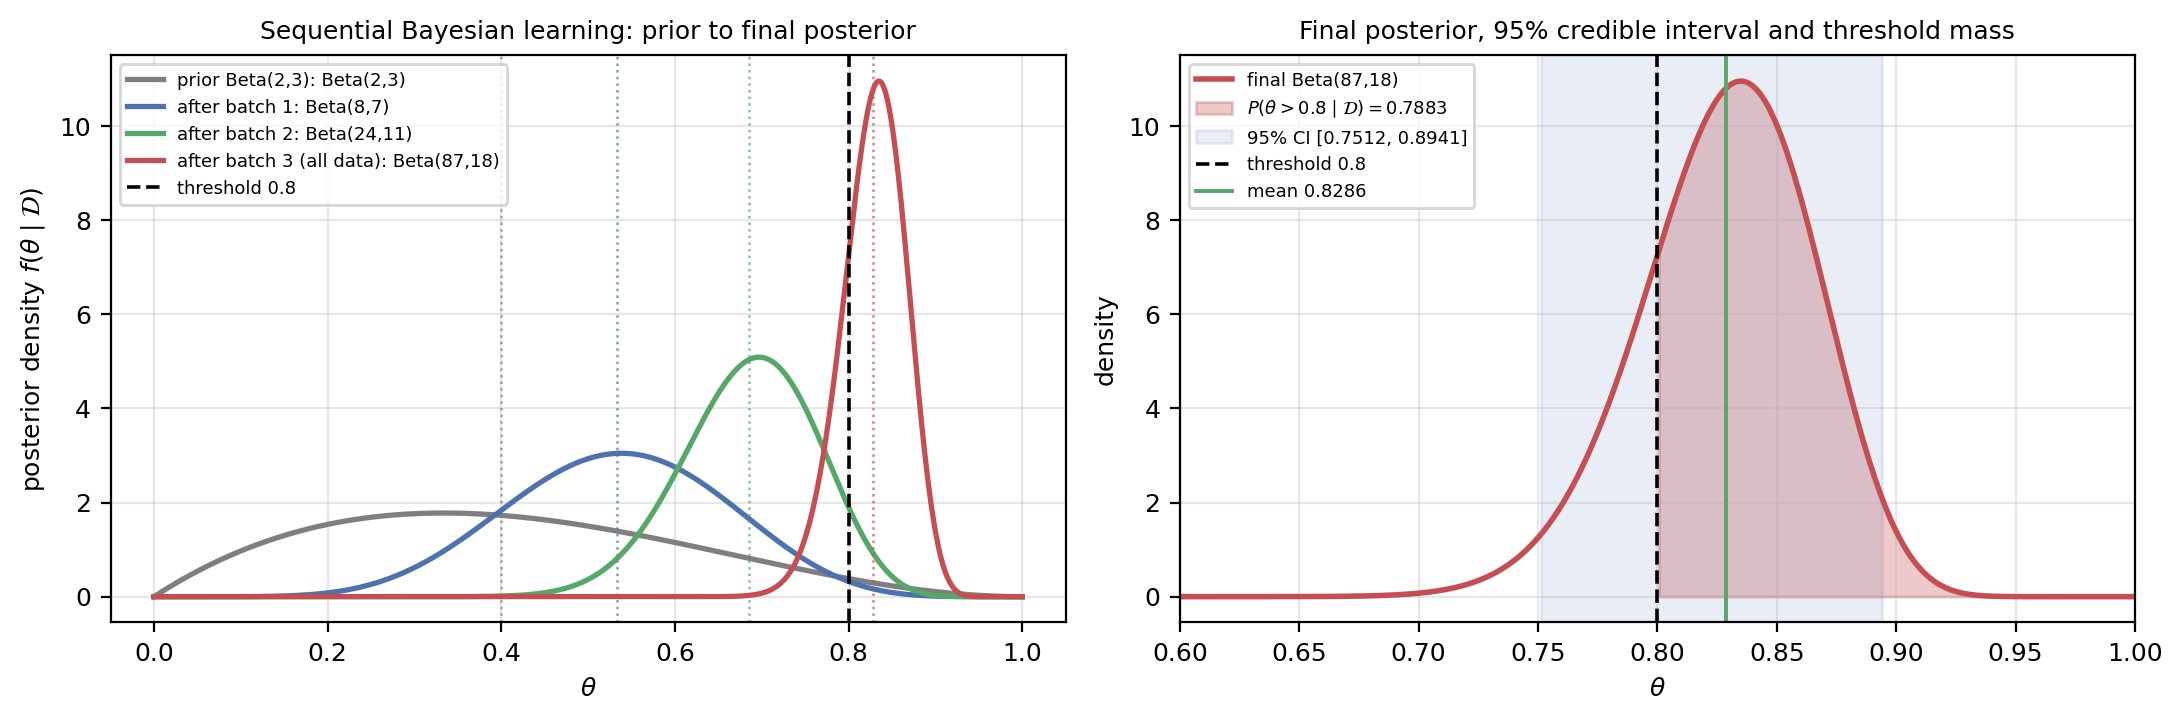
\includegraphics[width=0.385\textwidth]{../Satria_Pamungkas_21522611_COMP6010_Supplement/results/partB/B2_posterior_evolution.png}
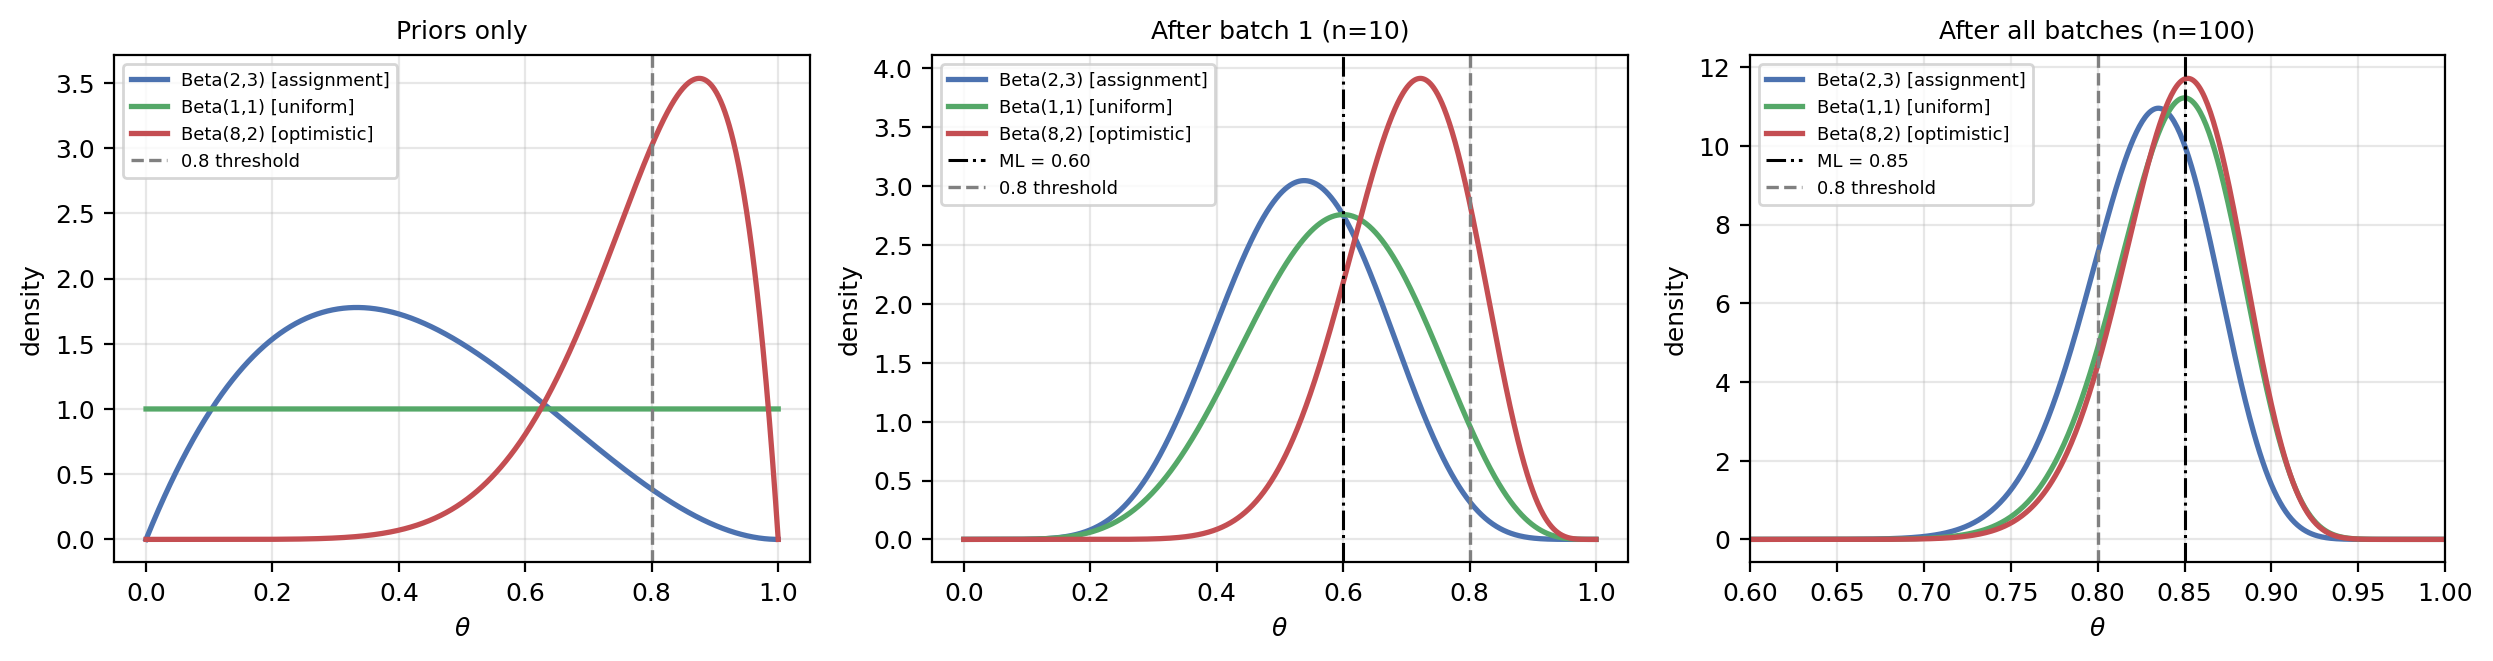
\includegraphics[width=0.385\textwidth]{../Satria_Pamungkas_21522611_COMP6010_Supplement/results/partB/B4_prior_sensitivity.png}
\caption{\textbf{Left:} learning batch by batch, then the final posterior with its 95\% interval and
the shaded area $P(\theta>0.8\mid\D)=0.7883$ --- clearly short of $0.95$ even though the average is
above $0.8$. \textbf{Right:} three different priors after 0, 10 and 100 attempts; they end up almost
on top of each other once enough data arrives.}
\label{fig:B}
\end{figure}

\subsection{B4. How much does the prior matter?}

\begin{table}[H]\centering\small
\caption{Prior sensitivity. After 10 attempts the three priors disagree a lot; after 100 they nearly
agree. \file{B4\_prior\_sensitivity.csv}}
\label{tab:Bprior}
\begin{tabular}{lccccccc}
\toprule
& \multicolumn{3}{c}{After batch 1 ($n{=}10$, ML $=0.600$)} & \multicolumn{3}{c}{After all batches ($n{=}100$, ML $=0.850$)} & \\
\cmidrule(lr){2-4}\cmidrule(lr){5-7}
Prior & Mean & MAP & $P(\theta{>}0.8)$ & Mean & MAP & $P(\theta{>}0.8)$ & Rule met? \\
\midrule
$\mathrm{Beta}(2,3)$ assignment & 0.5333 & 0.5385 & 0.0116 & 0.8286 & 0.8350 & 0.7883 & No \\
$\mathrm{Beta}(1,1)$ flat       & 0.5833 & 0.6000 & 0.0504 & 0.8431 & 0.8500 & 0.8811 & No \\
$\mathrm{Beta}(8,2)$ optimistic & 0.7000 & 0.7222 & 0.1631 & 0.8455 & 0.8519 & 0.9009 & No \\
\bottomrule
\end{tabular}
\end{table}

After batch 1 the priors are worth 5, 2 and 10 pretend attempts against only 10 real ones, so the means
spread from $0.533$ to $0.700$ and the threshold probabilities differ by a factor of 14 ($0.012$ to
$0.163$). After 100 attempts the data takes over: means bunch into $0.829$--$0.846$, a spread of only
$0.017$, all close to ML $=0.850$. The threshold probability stays more prior-sensitive than the mean
($0.788$--$0.901$), because it depends on the thin \emph{tail} rather than the middle --- worth knowing,
since a rule written as a tail probability is shakier under a change of prior than one written as an
average. The rule fails under all three priors, so that conclusion is safe; had it flipped, the honest
reading would be that the data are too weak to decide.

\textbf{ML and MAP with a flat prior.} With $\mathrm{Beta}(1,1)$ the prior is a flat line, so it
contributes nothing that varies with $\theta$, and maximising the posterior \emph{is} maximising the
likelihood: $\hat\theta_{\mathrm{MAP}}=\frac{(1+s)-1}{(1+s)+(1+n-s)-2}=\frac{s}{n}=\hat\theta_{\mathrm{ML}}$.
Confirmed in code at both stages ($0.600$ and $0.850$).

\textbf{Why that still does not make Bayes the same as ML.} They agree only about the single highest point of
the curve. The posterior \emph{mean} with a flat prior is $(1{+}s)/(2{+}n)=0.8431$, not $0.850$, and that mean
is the prediction for the next attempt --- so even with a flat prior the Bayesian \emph{prediction} differs from
ML. More importantly, ML returns one number while the posterior returns a whole curve, and both the credible
interval and $P(\theta>0.8\mid\D)$ come from that curve; ML cannot produce what the rule asks for. The gap
matters most when stakes are highest: with 5 successes out of 5, ML and MAP both say $\hat\theta=1.0$ ---
claiming the next attempt \emph{cannot} fail --- while the flat-prior prediction gives $0.857$ with interval
$[0.541,0.996]$. Picking a best value and carrying a distribution are different jobs, and only the second passes
uncertainty into the decision.

\section{Part C (option C2): drawing animals with flow matching}

\subsection{C1. The method and my two questions}

\textbf{Aim and data.} A model that generates $28\times28$ grey line drawings on request: give it a
category $y\in\{\textrm{cat},\textrm{dog},\textrm{fish}\}$ and random noise, and it produces a new
drawing of that animal. Data: Google Quick, Draw! bitmap files (CC BY 4.0, Google Creative Lab) [2], 4{,}000
original drawings per category.

\textbf{Flow matching in one idea.} Take a noise image $x_0$ and a real drawing $x_1$ and slide in a straight
line from one to the other. At time $t$ you are at
\[
x_t=(1-t)x_0+t\,x_1,\qquad\text{moving at speed}\qquad u_t=\frac{dx_t}{dt}=x_1-x_0,\qquad t\sim\mathcal{U}[0,1].
\]
Because the path is straight the speed is the \emph{same everywhere}, and it is just the difference between
the two ends. So I train a network $v_\theta(t,x_t,y)$ to predict it with ordinary squared error:
$\mathcal{L}_{\text{CFM}}(\theta)=\mathbb{E}\big\|v_\theta(t,x_t,y)-(x_1-x_0)\big\|^2$. Nothing is simulated
during training --- the correct answer is available directly. To generate, I start from fresh noise and follow
the predicted speeds from $t{=}0$ to $t{=}1$.

\begin{center}\small
\begin{tabular}{@{}l@{}}
\hline
\textbf{Training} (correct answer known in advance): \;
$x_0\sim\mathcal{N}(0,I)$, $x_1\sim p_{\text{data}}$, $t\sim\mathcal{U}[0,1]$
$\;\to\;x_t=(1{-}t)x_0{+}tx_1\;\to\;v_\theta(t,x_t,y)\;\xrightarrow{\ \text{squared error vs }x_1-x_0\ }\;\nabla_\theta$\\
\textbf{Generating} (follow the speeds forward): \;
$x_0\sim\mathcal{N}(0,I)\;\to\;\big[\,x\leftarrow x+\Delta t\cdot v_\theta(t,x,y)\,\big]\times n_{\text{steps}},\; t:0\to1\;\to\;x(1)=\text{drawing}$\\
\hline
\end{tabular}
\end{center}

One worry: the same halfway image $x_t$ could have come from many noise-and-drawing pairs, so which
speed is ``correct''? Squared error always settles on the \emph{average} answer, so the network learns
$\mathbb{E}[x_1-x_0\mid x_t,y]$ --- and flow matching's key result [4,5] is that following those average
speeds turns noise into the data distribution exactly. The network never guesses which pair it came
from; it learns the typical direction of travel, which is all generation needs.

\textbf{How this links to the unit.} The same three ingredients as Parts A and B. \emph{Known
structure:} the noise distribution and the straight-line path, both chosen by me. \emph{Unknown part
learned from data:} the speed field --- which, like the quantities in A and B, is an average.
\emph{Generating by sampling:} start from fresh noise and follow the path. The link to A4 is precise:
the straight line is a \emph{known} way to corrupt a drawing into noise, but knowing that forward
direction does not give me the way back, because the average speed depends on what real drawings look
like. That is the same trap as forcing evidence in a forward sampler and expecting the posterior.

\textbf{Q1 (a training setting).} Does training longer make drawings more recognisable, and does it cost
variety? \emph{Prediction:} a big jump from epoch 5 to 15, then flat; loss keeps falling; variety unchanged.
\textbf{Q2 (a generation setting).} How few steps can I get away with, and does the more careful midpoint
method beat plain Euler once network calls are counted fairly? \emph{Prediction:} few steps needed, levelling
off by 10--25, and at equal network calls midpoint gains little because straight paths barely bend.

\subsection{C2. What I built, and three key pieces of code}

\begin{table}[H]\centering\small
\caption{Baseline setup. Trained completely from scratch --- no pretrained weights, nothing frozen.
Implemented in PyTorch [8]; the reference implementation [6] was consulted for the 2-D starting point.
\file{C\_reproduction\_record.json}}
\label{tab:Cconf}
\begin{tabular}{@{}llll@{}}
\toprule
Data & 4{,}000 drawings/class $\times$ 3 & Network & \texttt{VelocityUNet} $28{\to}14{\to}7$, ch.\ $64{\to}128$ \\
Split & 9{,}600 train / 2{,}400 held out & Parameters & 1{,}838{,}081, all trainable \\
Preprocessing & $[0,255]\!\to\![-1,1]$, no resize & Conditioning & time + class, fed into every block \\
Augmentation & random flip, training set only & Optimiser & AdamW, lr $2\!\times\!10^{-4}$, cosine decay \\
Filtering & ink between 5\% and 55\% (8/20{,}700 cut) & Batch / epochs & 128 / 60, gradient clip 1.0 \\
Seeds & split+train \texttt{20260910}; 32 for generating & Hardware / time & RTX 3060 (12\,GB), \textbf{6.4 min} \\
\bottomrule
\end{tabular}
\end{table}

\textbf{(a) Building training examples --- \texttt{flow\_matching\_batch} in \texttt{flow\_model.py},
used inside \texttt{train()}.} \emph{In:} clean drawings \texttt{x1}, shape $(B,1,28,28)$. \emph{Out:} \texttt{(x\_t, t, target)}. It draws
noise \texttt{x0} of the same shape and one random time per image, reshaped so the same $t$ applies to every
pixel of that image, forms \texttt{x\_t = (1-t)*x0 + t*x1}, and returns \texttt{x1 - x0} as the target. Every
example uses fresh noise and time, so each drawing is seen at many noise levels.

\textbf{(b) Loss and weight updates --- the inner loop of \texttt{train()} in \texttt{train\_flow.py}.}
\emph{In:} a batch \texttt{(x1, y)}, the network, the optimiser. \emph{Out:} one update step. It applies
the flip augmentation (training set only), builds the three pieces above, then computes
\texttt{loss = mean((model(t,x\_t,y) - target)**2)}. That single line \emph{is} the flow-matching loss,
with the averaging over $t$ and noise done by the random batch, followed by
\texttt{zero\_grad}$\to$\texttt{backward}$\to$clip$\to$\texttt{step}. The whole generative model comes
down to a regression. \texttt{eval\_loss} uses a \emph{fixed} set of $t$ values so checkpoints compare
fairly instead of differing by luck.

\textbf{(c) Generating --- \texttt{sample\_ode} in \texttt{flow\_model.py}.} \emph{In:} the network, how many images, the labels, \texttt{n\_steps}, \texttt{method}, a \texttt{seed}.
\emph{Out:} the images, the \textbf{number of network calls (NFE)}, optionally the path. It seeds a generator,
draws $x_0$ --- \emph{the only random thing in the process} --- and steps $t{=}0$ to $1$. Euler uses one call
per step, midpoint two. I return the call count on purpose: comparing at the same \emph{number of steps} would
quietly give midpoint double the computing time.

\textbf{Checks before the long run.} I confirmed the shapes line up, that \emph{every} weight gets a gradient,
and specifically that the class embedding does --- if that connection breaks the loss still falls nicely while
every class produces the same picture, failing with no error message. I also checked the straight line starts
and ends where it should (differences around $10^{-7}$).

\begin{figure}[H]\centering
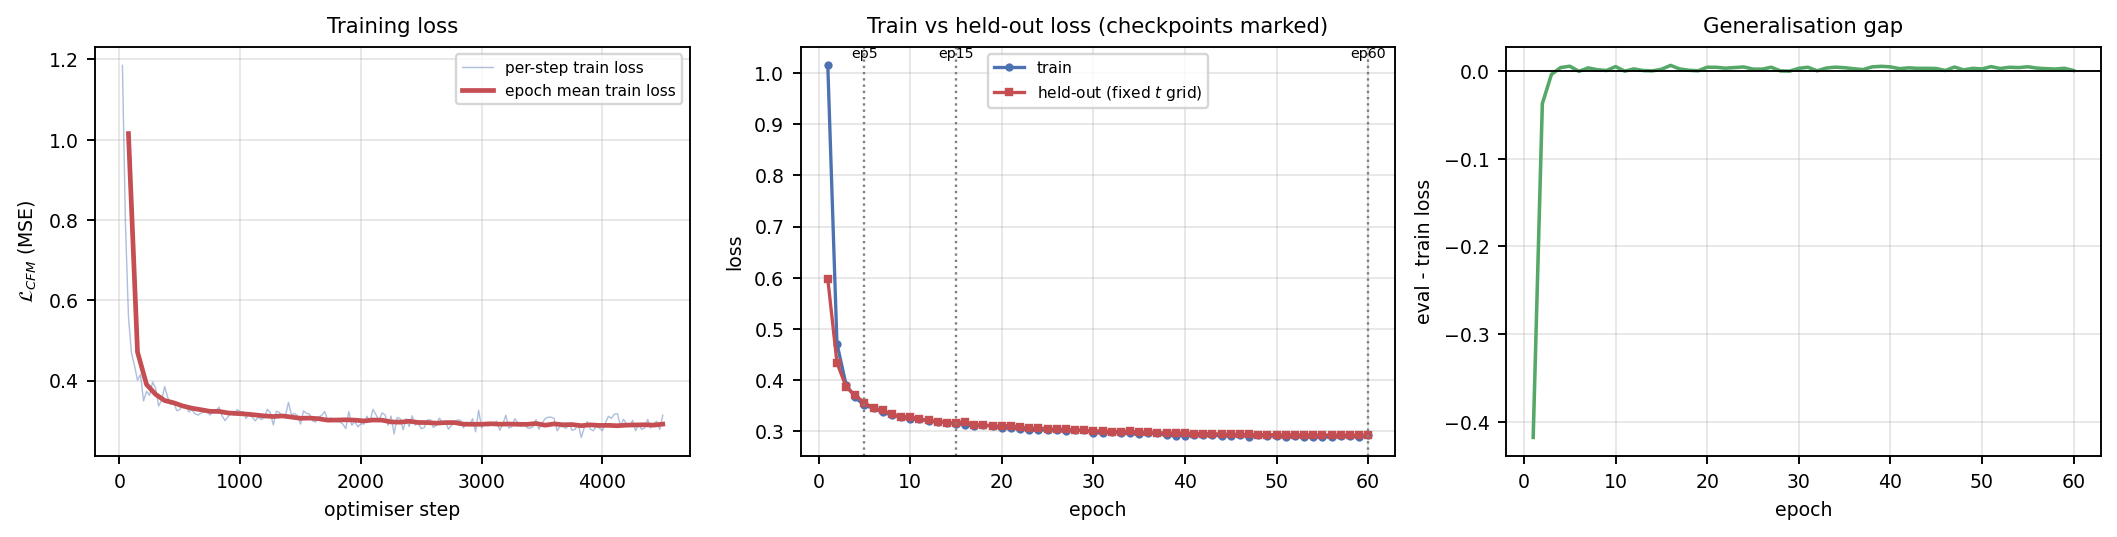
\includegraphics[width=0.49\textwidth]{../Satria_Pamungkas_21522611_COMP6010_Supplement/results/partC/C_training_curves.png}
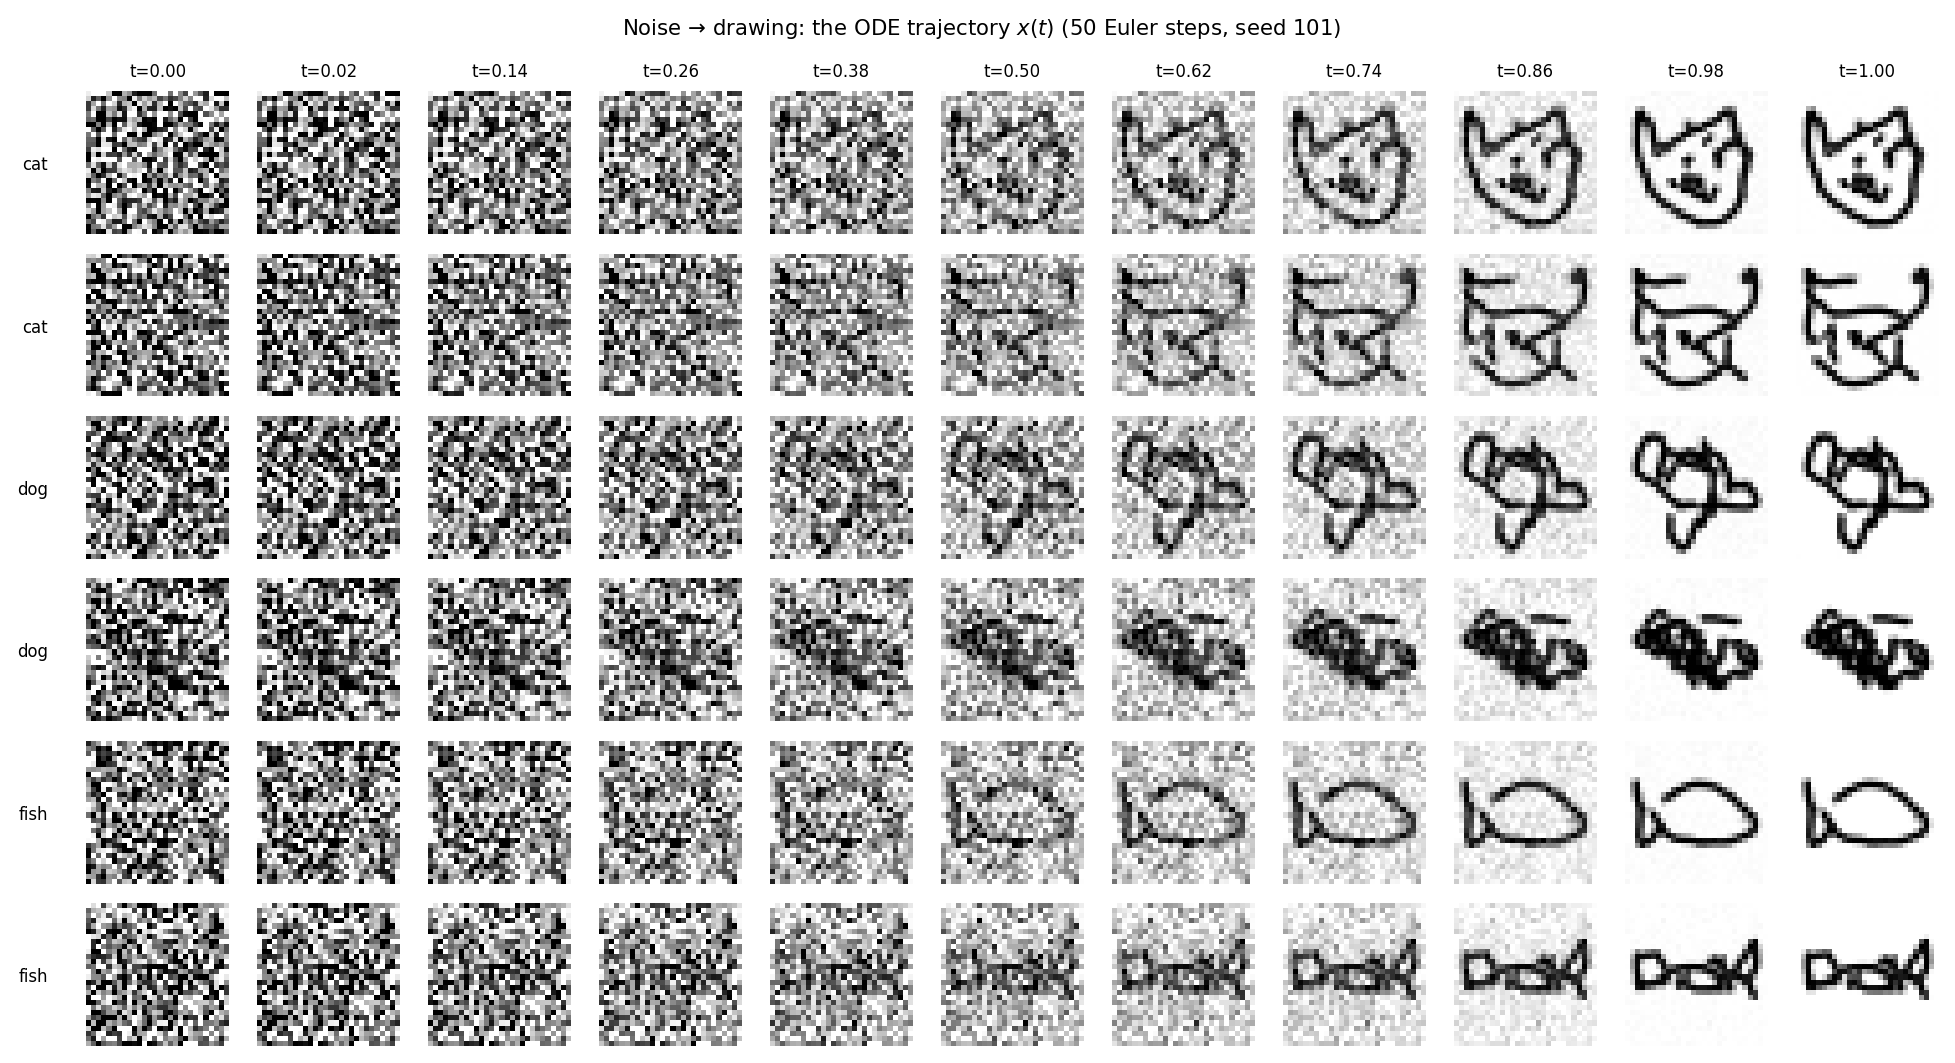
\includegraphics[width=0.335\textwidth]{../Satria_Pamungkas_21522611_COMP6010_Supplement/results/partC/C_trajectory_noise_to_drawing.png}
\caption{\textbf{Left:} training and held-out loss, with checkpoints marked. Held-out loss never rises
more than $0.006$ above training loss, so there is no overfitting at this size. \textbf{Right:} the
journey from noise to drawing. The rough shape is set by about $t{=}0.3$--$0.5$ and the later steps
just sharpen the lines --- what you would expect if the paths are nearly straight.}
\label{fig:Ctrain}
\end{figure}

\subsection{C3--C4. Controlled comparisons and scoring}

\textbf{The protocol.} I fixed a list of \textbf{32 seeds} once and reused it in \emph{every} comparison.
Each seed makes one drawing per class, so every setup gives \textbf{96 drawings} (32 per class, against
the required minimum of 16 and 4). I went above the minimum on purpose: a first run with 8 seeds gave an
identical $0.75$ for all three checkpoints, the score simply being too coarse to tell them apart. Only
one thing changes at a time. \textbf{The quality score} is \emph{recognisability}: the share of a setup's
96 drawings that a separate small CNN files under the class I \emph{asked for}. That CNN is trained
\emph{only on real held-out drawings} the generator never saw, and scores \textbf{0.8375} on them --- so
$0.8375$, not $1.0$, is the realistic maximum.

\begin{table}[H]\centering\small
\caption{Both comparisons. The margin of error is $\pm0.041$ throughout ($n{=}96$), so any gap under
about $0.09$ means nothing. \file{C\_all\_results.csv}}
\label{tab:Cres}
\begin{tabular}{@{}llrrrrrr@{}}
\toprule
& Setup & Held-out loss & Recog.\ ($\pm$0.041) & Confidence & Variety & NFE/img & ms/img \\
\midrule
\multirow{4}{*}{\rotatebox{90}{\scriptsize training}}
& epoch 5   & 0.3557 & 0.781 & 0.637 & 22.6 & 50 & 16.9 \\
& epoch 15  & 0.3164 & 0.771 & 0.672 & 22.1 & 50 & 16.9 \\
& epoch 60 (baseline) & 0.2922 & \textbf{0.802} & \textbf{0.704} & 22.5 & 50 & 16.9 \\
& epoch 60, \emph{quarter} of the data & 0.3297 & 0.760 & --- & 22.1 & 50 & 16.9 \\
\midrule
\multirow{6}{*}{\rotatebox{90}{\scriptsize generating}}
& Euler 2 steps    & --- & 0.781 & 0.630 & \textbf{14.9} & 2 & 0.78 \\
& Euler 5 steps    & --- & 0.792 & 0.703 & 20.6 & 5 & 1.78 \\
& Euler 10 steps   & --- & 0.792 & 0.706 & 21.7 & 10 & 3.4 \\
& Euler 50 steps   & --- & 0.802 & 0.704 & 22.5 & 50 & 16.9 \\
& Euler 100 steps  & --- & 0.792 & 0.702 & 22.6 & 100 & 33.7 \\
& Midpoint 5 steps & --- & 0.802 & 0.707 & 22.7 & 10 & 3.5 \\
\bottomrule
\end{tabular}
\end{table}

\begin{figure}[tp]\centering
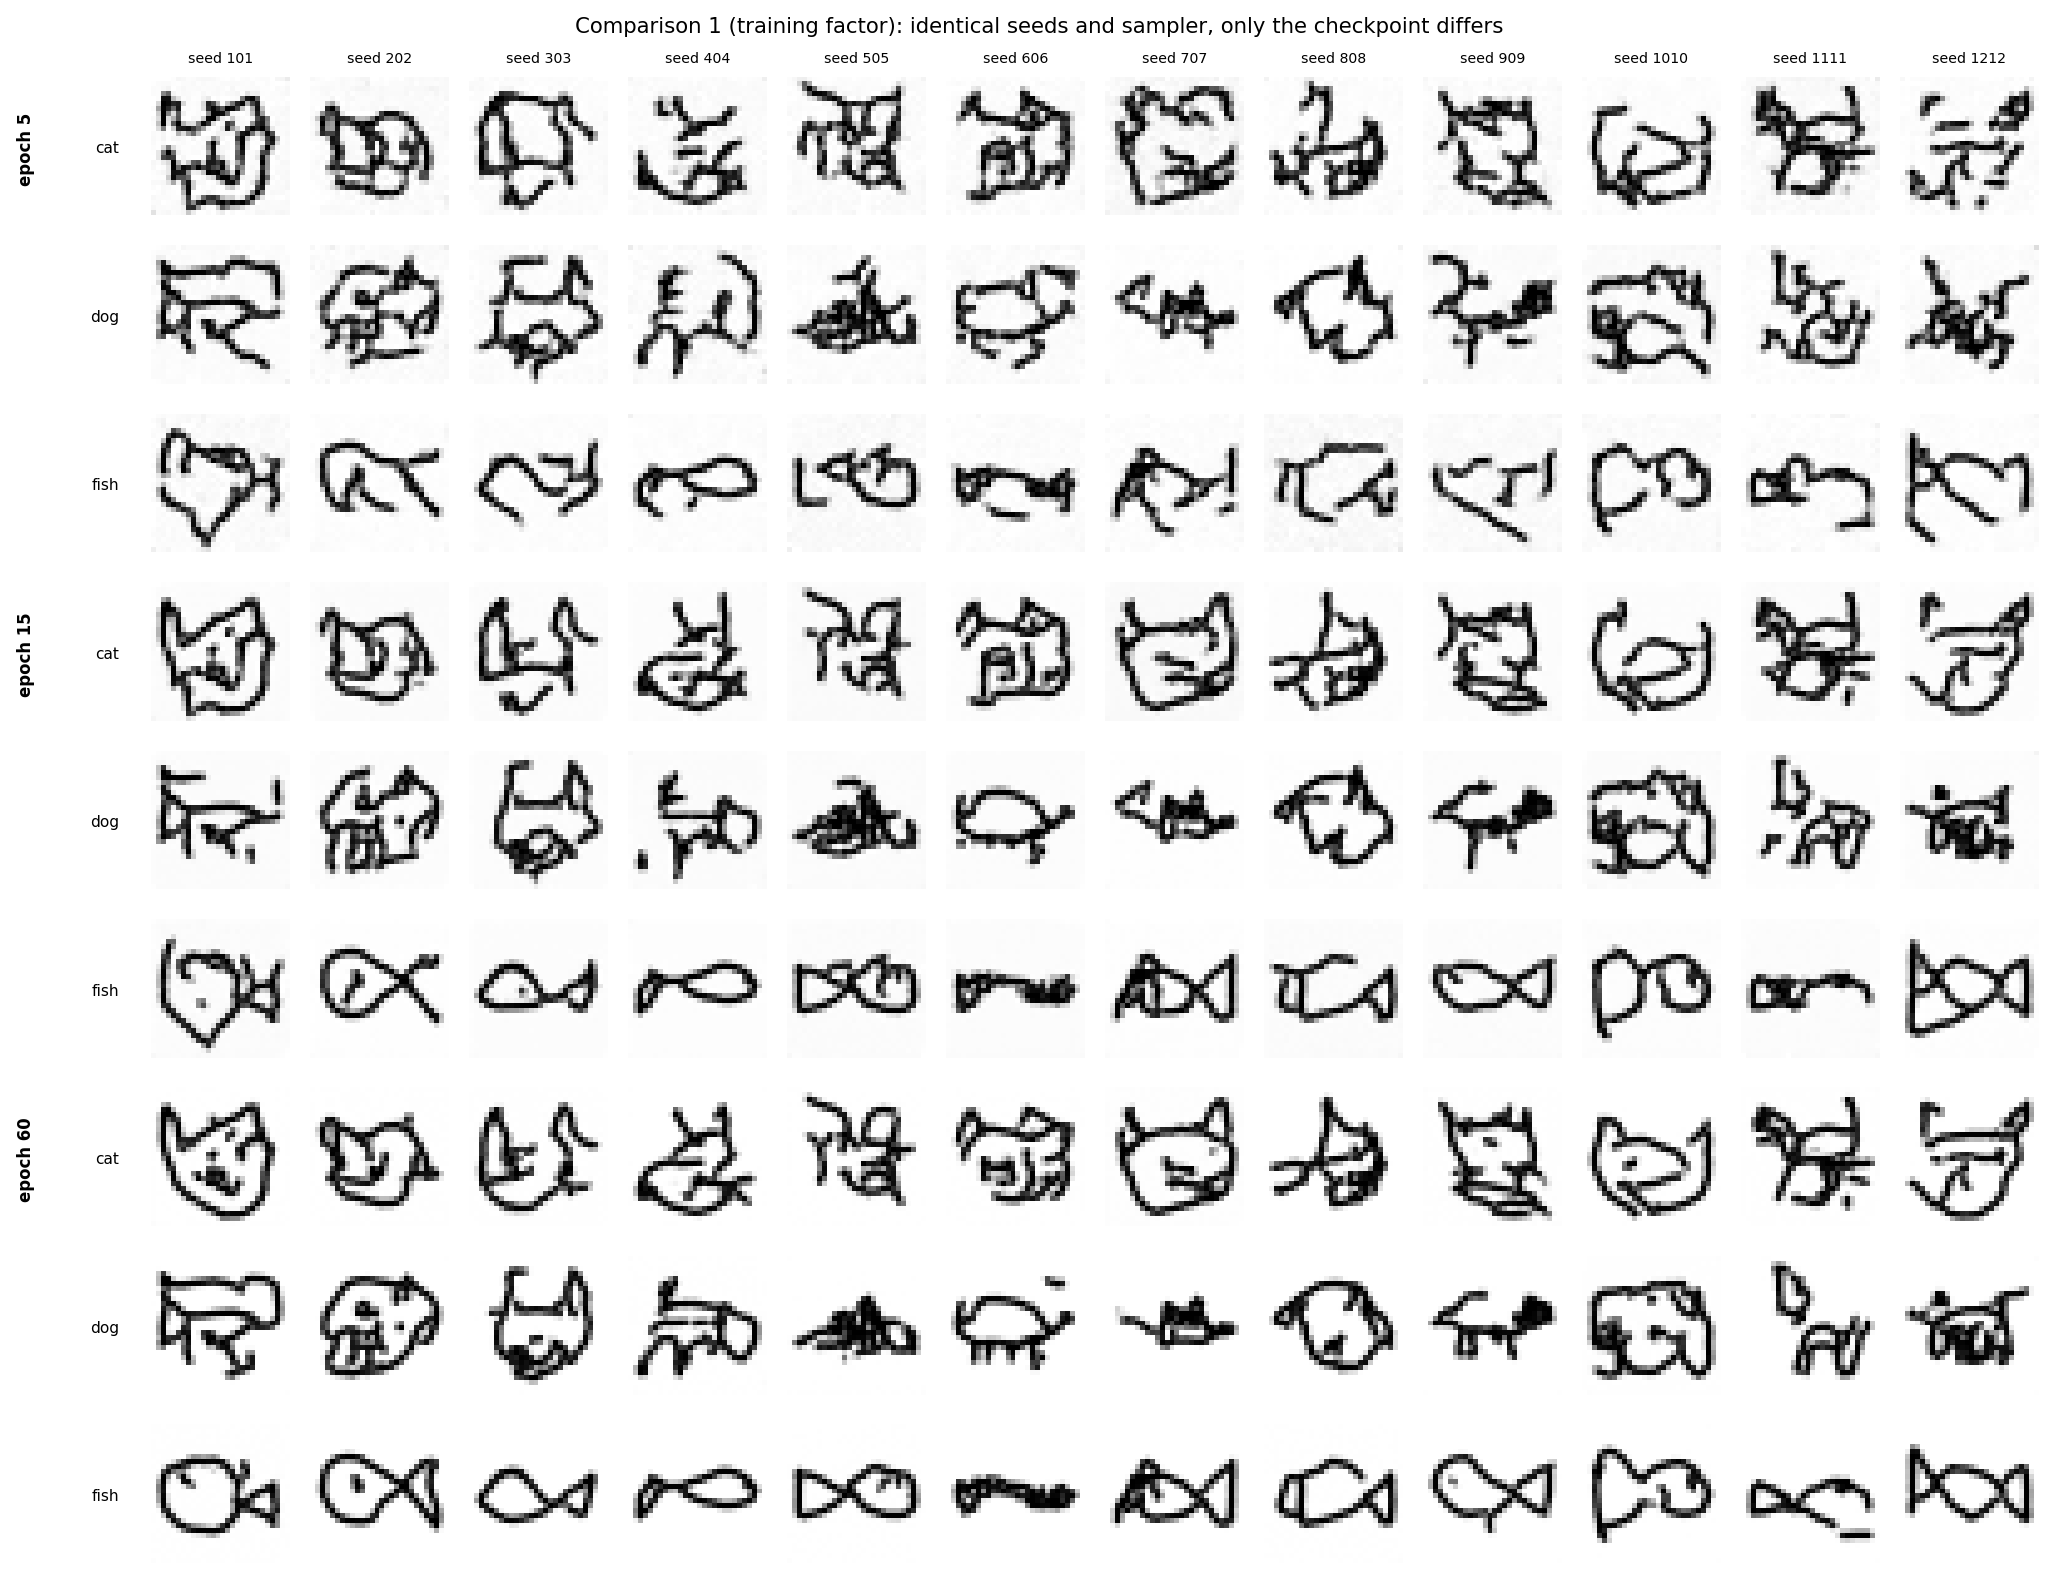
\includegraphics[width=0.355\textwidth]{../Satria_Pamungkas_21522611_COMP6010_Supplement/results/partC/C_matched_grid_checkpoints.png}
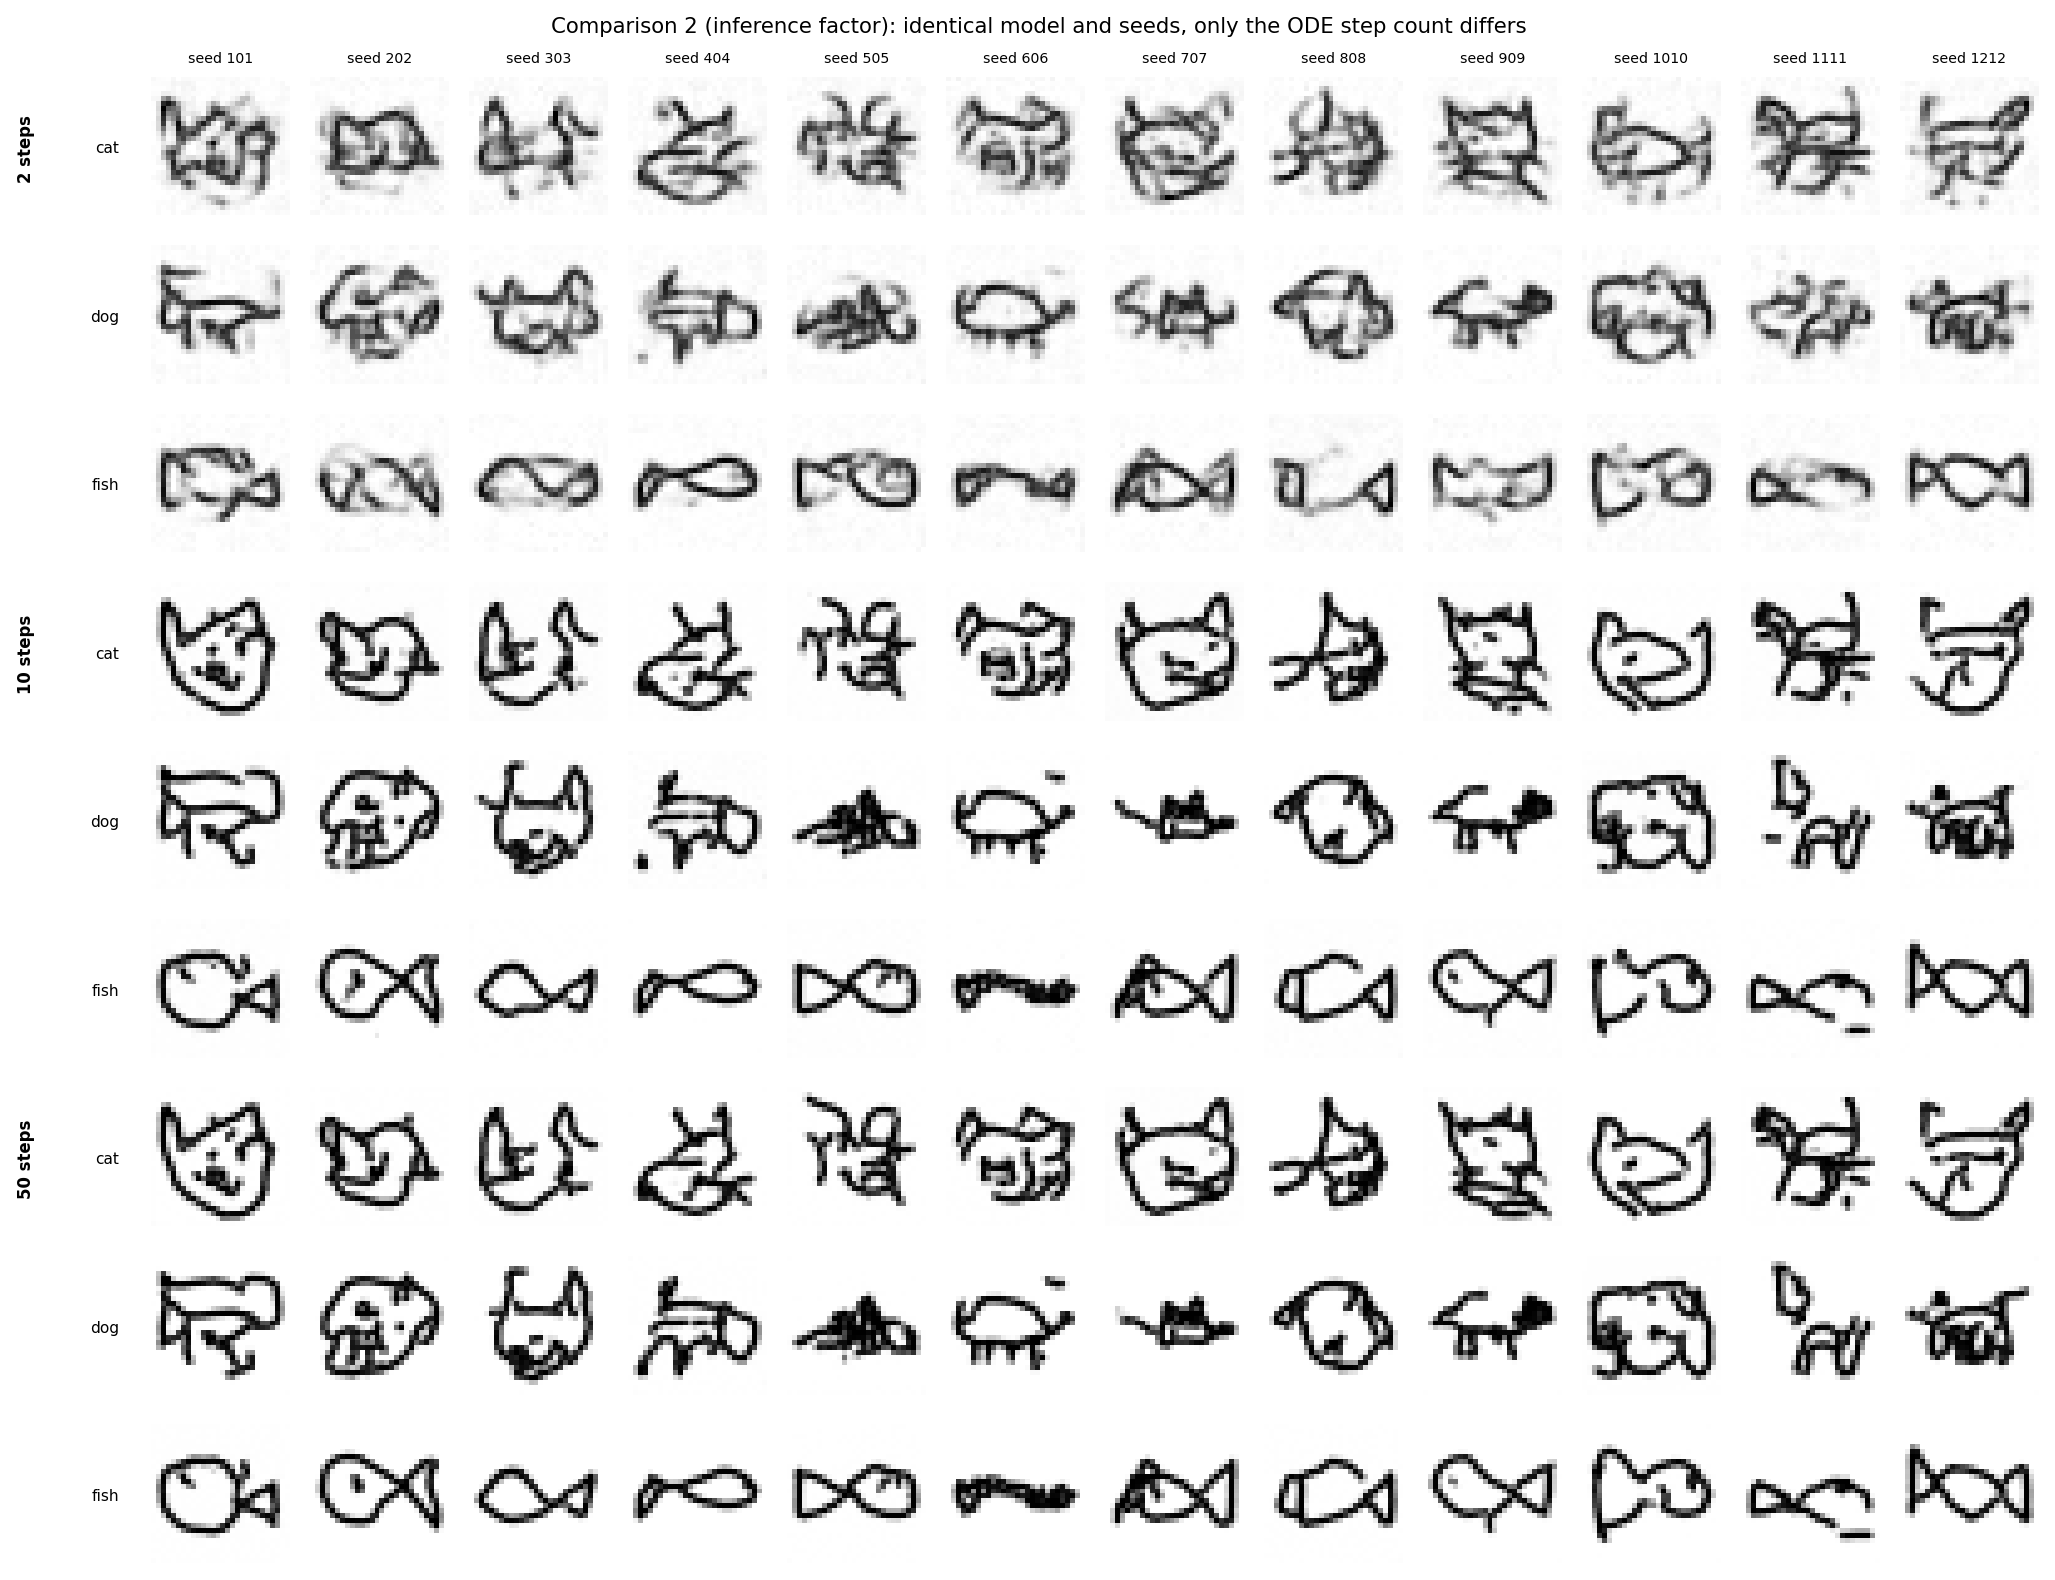
\includegraphics[width=0.355\textwidth]{../Satria_Pamungkas_21522611_COMP6010_Supplement/results/partC/C_matched_grid_steps.png}
\caption{Matched grids with the same seeds down each column, showing the first 12 of 32 seeds, failures
included. \textbf{Left (Q1):} only the checkpoint changes. The drawings clearly get better by eye ---
epoch-5 cats are scribbly, epoch-60 cats have clean ears and faces --- even though the
recognisability \emph{score} hardly moved. \textbf{Right (Q2):} only the number of steps changes. The
2-step row is visibly faint and washed out, while 10 and 50 steps look almost the same. All 96
drawings for all 14 setups, including raw \texttt{.npz} arrays, are in
\file{results/partC/sample\_grids/}.}
\label{fig:Cgrids}
\end{figure}

\subsection{C5. What the results mean}

\textbf{Q1: my prediction was wrong, and how it was wrong is the most useful finding here.} Held-out loss
dropped steadily by 18\% ($0.356\to0.292$) and average confidence rose steadily ($0.637\to0.704$), but
\emph{recognisability barely moved}: $0.781\to0.771\to0.802$, half the margin of error. I cannot claim a real
gain from training 12 times longer. Three things follow. \emph{First}, this is a clear numerical demonstration
that \textbf{training loss does not measure picture quality}: the loss averages speed errors over all times
$t$, and most of the leftover improvement happens at noise levels that barely affect where the path lands.
\emph{Second}, confidence was the more sensitive measurement --- it rose steadily while yes/no scoring throws
that information away, so longer training sharpens drawings that were \emph{already} classified correctly.
Reporting only the score would have hidden a real effect; reporting it \emph{as if} it showed one would have
invented an effect. \emph{Third}, the task levels off early: by epoch 5 (32 seconds) drawings already score
$0.781$ against a maximum of $0.8375$. Figure~\ref{fig:Cgrids} shows the drawings really \emph{do} get better,
so the honest conclusion is that my \emph{measurement} was too blunt here, not that training does nothing.
Per-class numbers locate the difficulty: \texttt{fish} scores $0.94$--$0.97$ at every checkpoint while
\texttt{dog} scores $0.53$--$0.66$, matching the classifier's own limits on real drawings (fish $0.916$, cat
$0.821$, dog $0.781$) --- dogs are hardest for scorer and generator alike, so this is the data, not broken
conditioning. The \emph{data-size} comparison does move things: quartering the training set at identical
training time pushes held-out loss $0.292\to0.330$ and recognisability $0.802\to0.760$, so at this network
size the limit is data, not training time.

\textbf{Q2: both halves of my prediction held, and the levelling-off is even more extreme than expected.}
Recognisability is flat from 2 to 100 Euler steps, all within one margin of error. What \emph{does} change
at 2 steps is \textbf{variety}, collapsing from about $22.5$ to $\mathbf{14.9}$ --- a 34\% drop, far
bigger than any wobble elsewhere --- with confidence also falling to $0.630$. So the 2-step failure is not
``wrong animal'' but ``not finished'': drawings land roughly in the right place yet come out faint and too
similar, exactly as Figure~\ref{fig:Cgrids} (right) shows. Past about 5 steps, extra steps buy nothing
measurable while cost climbs linearly --- $0.78$\,ms to $33.7$\,ms per image from 2 to 100 steps, 43 times
the cost for no gain. This is flow matching's practical advantage over diffusion sampling [7]: straight-line
training gives nearly straight paths, so a handful of steps is enough where diffusion needs hundreds.
Comparing solvers \textbf{at equal network calls}, the differences are $+0.010$, $-0.010$ and $0.000$,
each far below the $\pm0.058$ margin of error, so none is distinguishable. That fits the geometry: a more
careful solver only pays off when the path bends, and these are trained nearly straight. Midpoint's only
visible edge is at the cheapest setting, recovering variety $23.7$ on 4 network calls against Euler's
$14.9$ on 2. \file{C\_comparison2\_matched\_nfe.csv}

\textbf{Why the output is still random when the solver is not.} Both solvers are fixed recipes: pin down
$x_0$ and the output is pinned down too, which is what makes my 32-seed list repeatable. All randomness
enters through the \emph{starting noise} $x_0$; the path just carries the noise distribution onto the
drawing distribution. Variety comes from where you start, not from anything added along the way --- the
real difference from a diffusion sampler [7], which adds new randomness every step. I checked this rather than
assuming it, and the check caught something: with default settings two runs of the \emph{same} seed differed by
about $7\times10^{-4}$, because the GPU library may pick different convolution algorithms each time. The maths
was never at fault ($x_0$ was identical), but ``same seed, same picture'' held only to plotting accuracy until I
pinned the GPU settings (\texttt{enable\_deterministic()}). Now same-seed runs match exactly, and the notebook
checks it.

\textbf{Copying.} The average distance from each of the 96 generated drawings to its closest
\emph{training} drawing is \textbf{16.62}, against \textbf{15.69} for 200 real \emph{held-out} drawings
measured the same way --- so generated drawings are actually \emph{further} from the training set than
genuinely unseen real drawings, which argues against copying. The six closest pairs share only a rough
layout (a body outline, a tail pointing the same way), not the strokes. Looking similar is not proof:
with 3{,}200 simple doodles per class, any believable new cat \emph{has} to resemble some training cat,
so the meaningful comparison is the spread of distances, not a single pair.
\file{C\_memorisation\_distances.csv}

\textbf{Limits of my score, and of the study.}
(i) The realistic maximum is $0.8375$, not $1.0$, because the doodles are often unclear even to a person;
epoch 60 reaches 96\% of it. (ii) The scoring CNN has biases of its own, so a good score is necessary but not
sufficient for ``a person would call this a cat''. (iii) \textbf{It measures whether the class is right, not
whether the drawing is good, and this caught me out}: the 2-step drawings scored $0.781$, indistinguishable
from 50 steps, despite being obviously worse and losing 34\% of their variety --- nearly blind to the biggest
quality difference in the study. (iv) With 96 drawings the margin of error is $0.041$, so gaps under about
$0.09$ cannot be resolved; only two effects beat the noise (the variety collapse at 2 steps, the loss worsening
on a quarter of the data) and the rest are genuine null results. Finding smaller effects needs several hundred
drawings per setup --- affordable at 17\,ms each, and the first thing I would change. (v) Straight-line distance
between images is weak: fine for near-duplicates, blind to a copy shifted a few pixels. (vi) $28\times28$ line
drawings are the easy end of image generation, and nothing here shows the method scales to photographs. I did
not compute FID or run a human study --- both need far more samples or a pretrained feature extractor.

\begin{figure}[tp]\centering
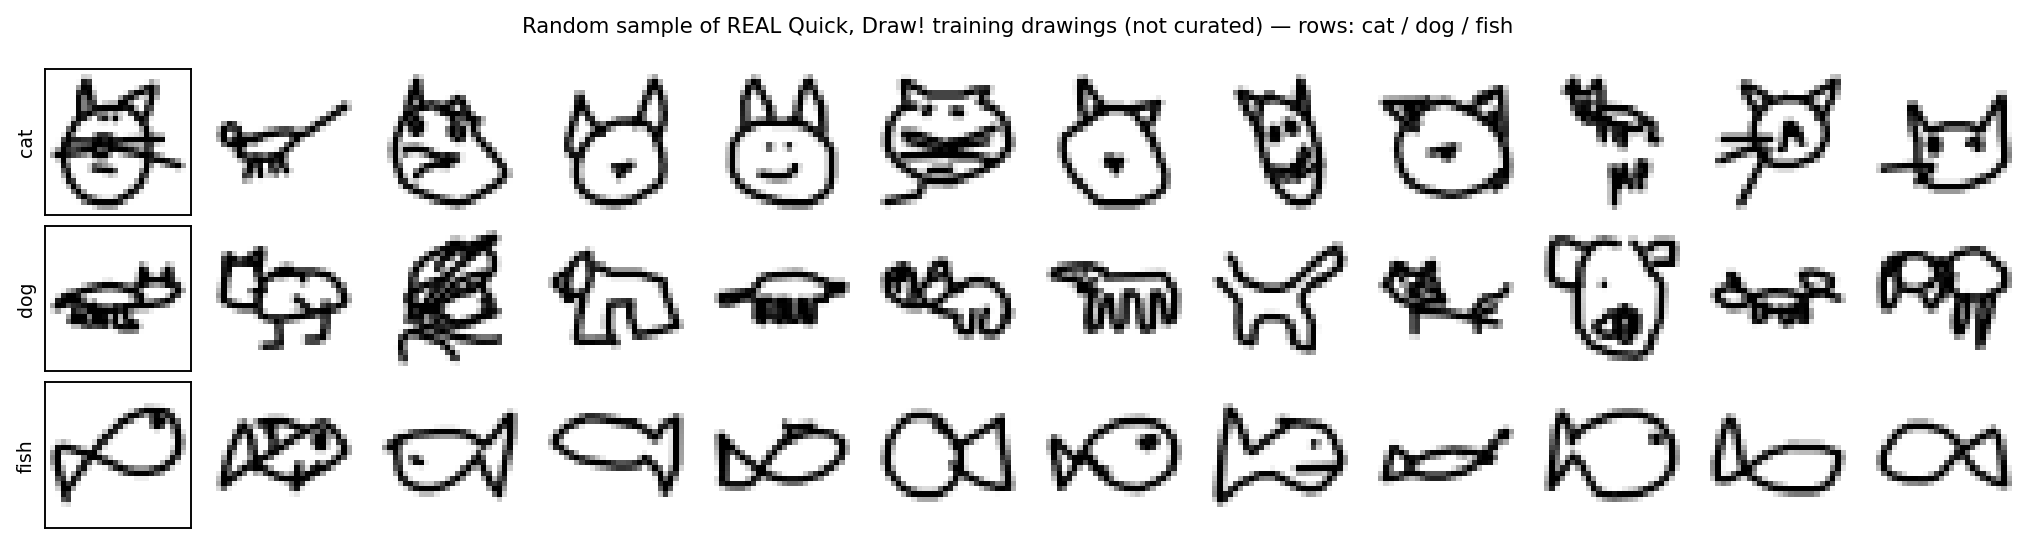
\includegraphics[width=0.50\textwidth]{../Satria_Pamungkas_21522611_COMP6010_Supplement/results/partC/C_real_data_grid.png}
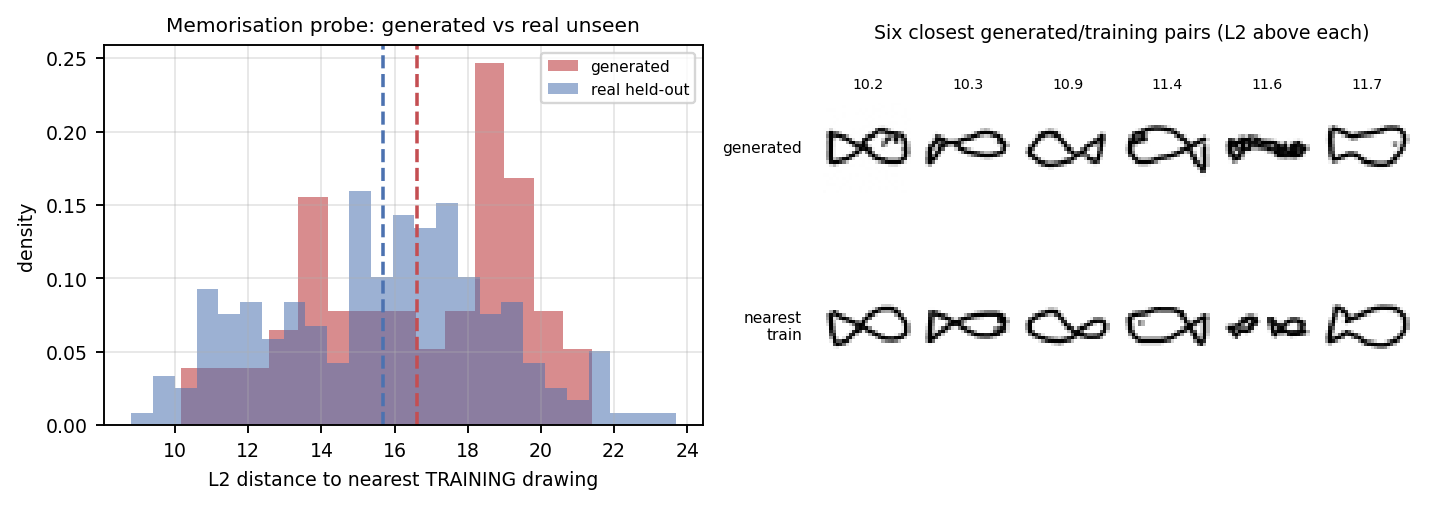
\includegraphics[width=0.315\textwidth]{../Satria_Pamungkas_21522611_COMP6010_Supplement/results/partC/C_memorisation_probe.png}
\caption{\textbf{Left:} a random (not hand-picked) sample of the real \emph{training} drawings, looked
at before training. Several are unclear even to a person --- they are 20-second public doodles --- and
that is what sets the $0.8375$ ceiling rather than $1.0$. \textbf{Right:} the copying check. Generated
drawings sit at average distance $16.62$ from their closest training drawing versus $15.69$ for real
held-out drawings, and even the six closest pairs share only a rough layout, not strokes.}
\label{fig:Cdata}
\end{figure}

\section{Conclusion: inference $\rightarrow$ learning $\rightarrow$ generating}

Part~A used a \emph{fully known} model, where the only real difficulty was handling evidence properly:
overwriting later evidence gave back the prior ($0.0799$ against the true $q_2=0.2933$), and rejection sampling
and likelihood weighting are the two valid repairs. Part~B kept the structure known but made \emph{one number}
unknown, and learning a full curve over it changed the decision: ML $=0.850$ sits above the threshold, yet
$P(\theta>0.8\mid\D)=0.788$ fails the $0.95$ rule, because a single number throws away the very width the rule
is about. Part~C made the unknown a whole \emph{function}: I chose the noise distribution and the path, and the
network learned the speed field --- like the quantities in A and B, just an average. Generating is then sampling
in the same sense: draw from something simple and push it through what was learned. The thread through all three
is that a generative model is not a different \emph{kind} of thing from a Bayesian network --- it is the same
split-up, learn, sample pattern with a network in place of a probability table, and the same warning applies at
every size: knowing the forward direction never gives you the reverse for free. Part~C added the lesson the brief
points at: an 18\% better training loss produced no measurable change in drawing quality, so the measurement you
pick decides what you can conclude.

\section*{AI-use statement}

I used Claude (Anthropic), model Opus 5, through the Claude Code CLI on 9--10 September 2026, for explanations
of flow matching, code scaffolding for the network and sampler, notebook structure and debugging. All the maths,
experiment design, checking and claims are my own responsibility, and every number reported came from code I ran
on my own machine. Five interactions are written up in \texttt{AI\_USE\_LOG.md} with the prompt, the relevant
reply, my check and what I decided. They include one independently verified correctness check (I re-derived
Part~A's exact answers with a separate brute-force program, agreeing to 10 decimal places, and added a
swapped-table test the assistant had not suggested, showing the total-adds-to-1 check is weaker than it looks)
and one prediction-versus-result comparison (the Euler/midpoint expectation above, which the data contradicted).
I also record one suggestion I \textbf{rejected}: the proposed ink-filter limits of 2\% and 60\% cut out
\emph{nothing} once I measured the real distribution, so I recalibrated to 5\% and 55\%. The log's table lists all
16 checks I ran. No result, runtime, citation or figure in this submission was made up.

\section*{References}
\scriptsize
\begin{enumerate}[leftmargin=1.4em,itemsep=0pt]
\item COMP6010 teaching materials (2026): \emph{Bayesian Networks I}; \emph{Bayesian Networks 2 --
Inference}; \emph{Learning Probabilistic Models}; \emph{Diffusion and Flow Matching Models};
continuous-probability notes; Practicals 1--4, 6 and 7. Primary source for all three parts.
\item Google Creative Lab. \emph{The Quick, Draw! Dataset} (bitmap format), CC BY 4.0.
github.com/googlecreativelab/quickdraw-dataset. Categories \texttt{cat}, \texttt{dog}, \texttt{fish} retrieved 10 Sept 2026; checksums in \texttt{C\_data\_manifest.json}.
\item SciPy documentation, \texttt{scipy.stats.beta} (v1.15.3) --- Beta densities, cumulative
functions, quantiles and sampling.
\item Lipman, Y., Chen, R.T.Q., Ben-Hamu, H., Nickel, M., Le, M. (2023). Flow Matching for Generative
Modelling. \emph{ICLR}. arXiv:2210.02747
\item Liu, X., Gong, C., Liu, Q. (2023). Flow Straight and Fast: Learning to Generate and Transfer Data
with Rectified Flow. \emph{ICLR}. arXiv:2209.03003
\item Meta AI. \emph{flow\_matching} library and example notebooks.
github.com/facebookresearch/flow\_matching
\item Ho, J., Jain, A., Abbeel, P. (2020). Denoising Diffusion Probabilistic Models. \emph{NeurIPS}. arXiv:2006.11239 --- used for the comparison in \S C5.
\item Paszke, A.\ et al.\ (2019). PyTorch (v2.10.0+cu128).
\item Kish, L. (1965). \emph{Survey Sampling}. Wiley --- effective sample size used in \S A4.
\end{enumerate}

\end{document}
